\section{Introduction}
%A brief review on field design in HV equipment.
The design of electrical equipment always involves an aspect of insulation design.
For the safe and efficient operation of electrical equipment it is necessary to have an electrical circuit and a means of isolating this circuit from the surrounding environment \cite{warne2005newnes}.
Power systems contain a complex structure of generators, transmission lines, transformers, switchgear and more. 
All of these different devices require an appropriately selected insulation material in order to isolate the mechanical casings and support structures from the high voltage components \cite{james2008condition}.

The purpose of this report is to describe the design and simulation of a high voltage bushing. Bushings are an integral part of power system insulation. 
IEEE standard C57.19.00 describes a bushing as ``an insulating structure, including a through conductor or providing a central passage for such a conductor, with provision for mounting on a barrier, conducting or otherwise, for the purpose of insulating the conductor from the barrier and conducting current from one side of the barrier to the other.''\cite{1440990}.
Bushings are required for situations such as connecting the external conductor to the internal windings of a transformer through the walls of the metal oil tank.
The walls of the transformer housing will be grounded, but need to be shielded from the incoming high voltage conductor, hence the use of a bushing \cite{warne2005newnes}.
An example of this usage can be seen in figure \ref{Figure:BothBushPics}, as 400kV grid conductors enter an oil filled transformer casing.
The shedding on the outer cylinder can be seen in figure \ref{Figure:BothBushPics} which helps increase electrical strength in wet conditions.

\begin{figure}[!htb]
  \centering
  \subfigure[Transformer wall connection]{
    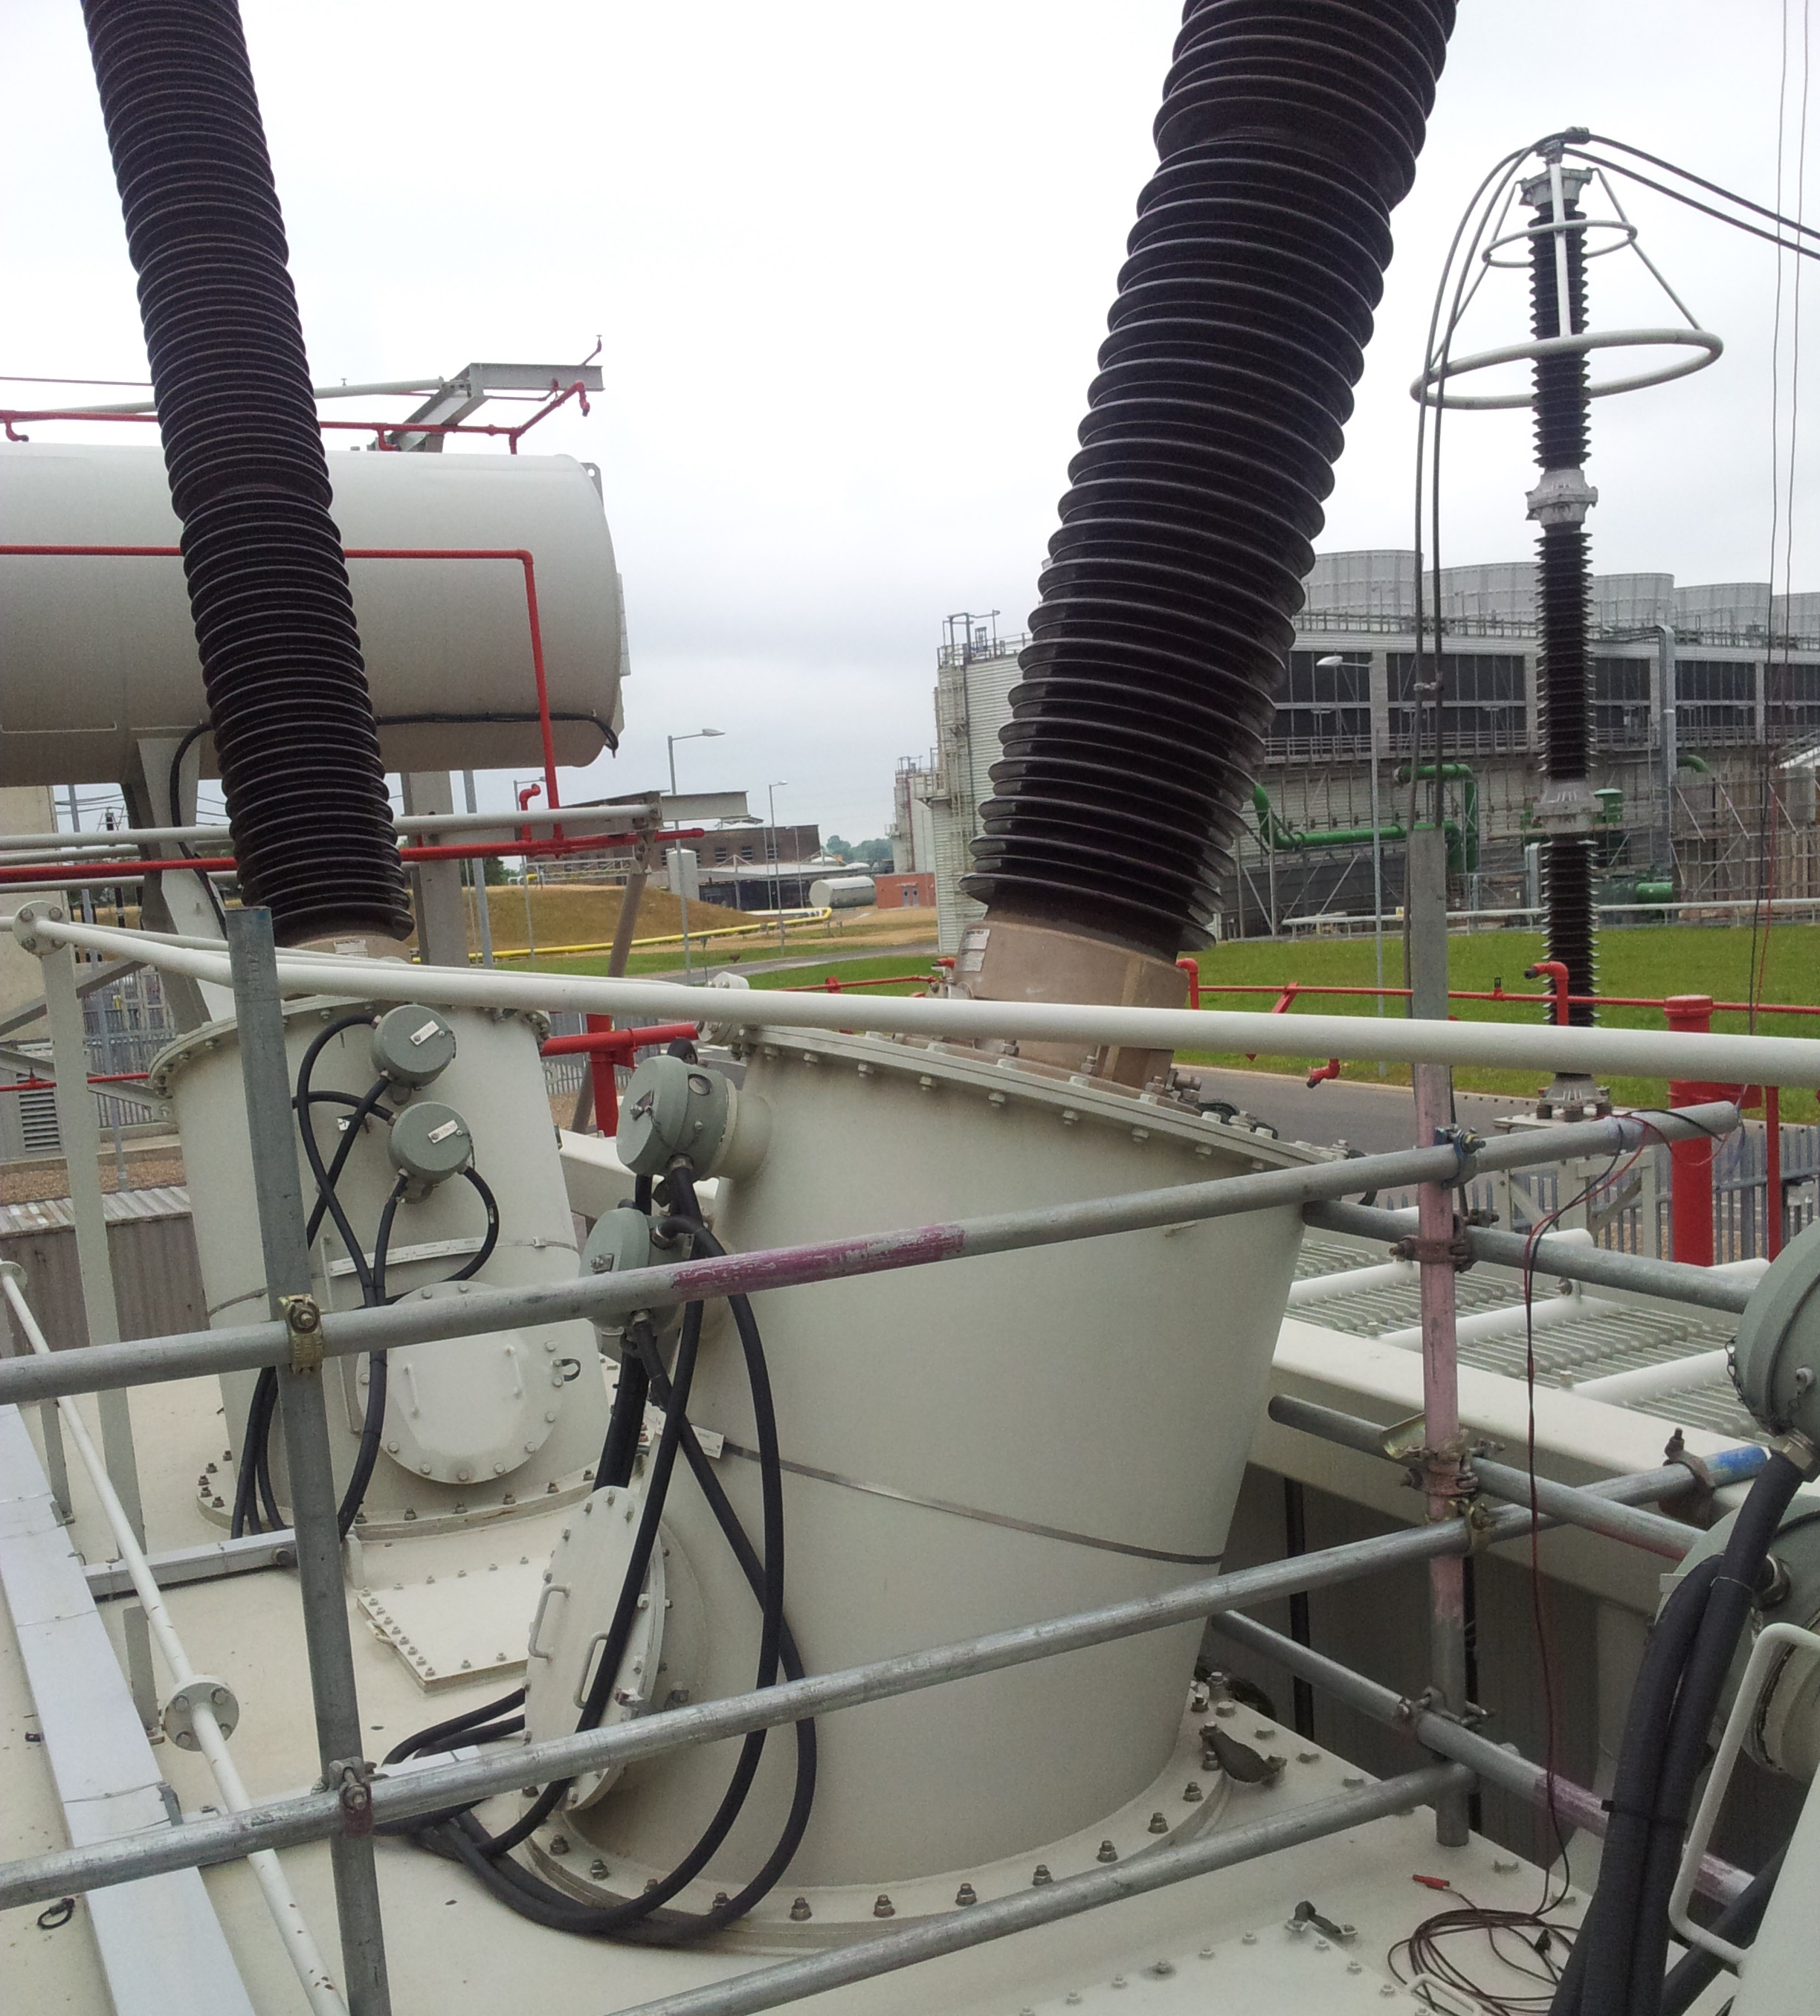
\includegraphics[height = 6cm]{StaythorpeHVBushing.jpg} 
	\label{Figure:Bush1}
  }
  \subfigure[Wide view]{
    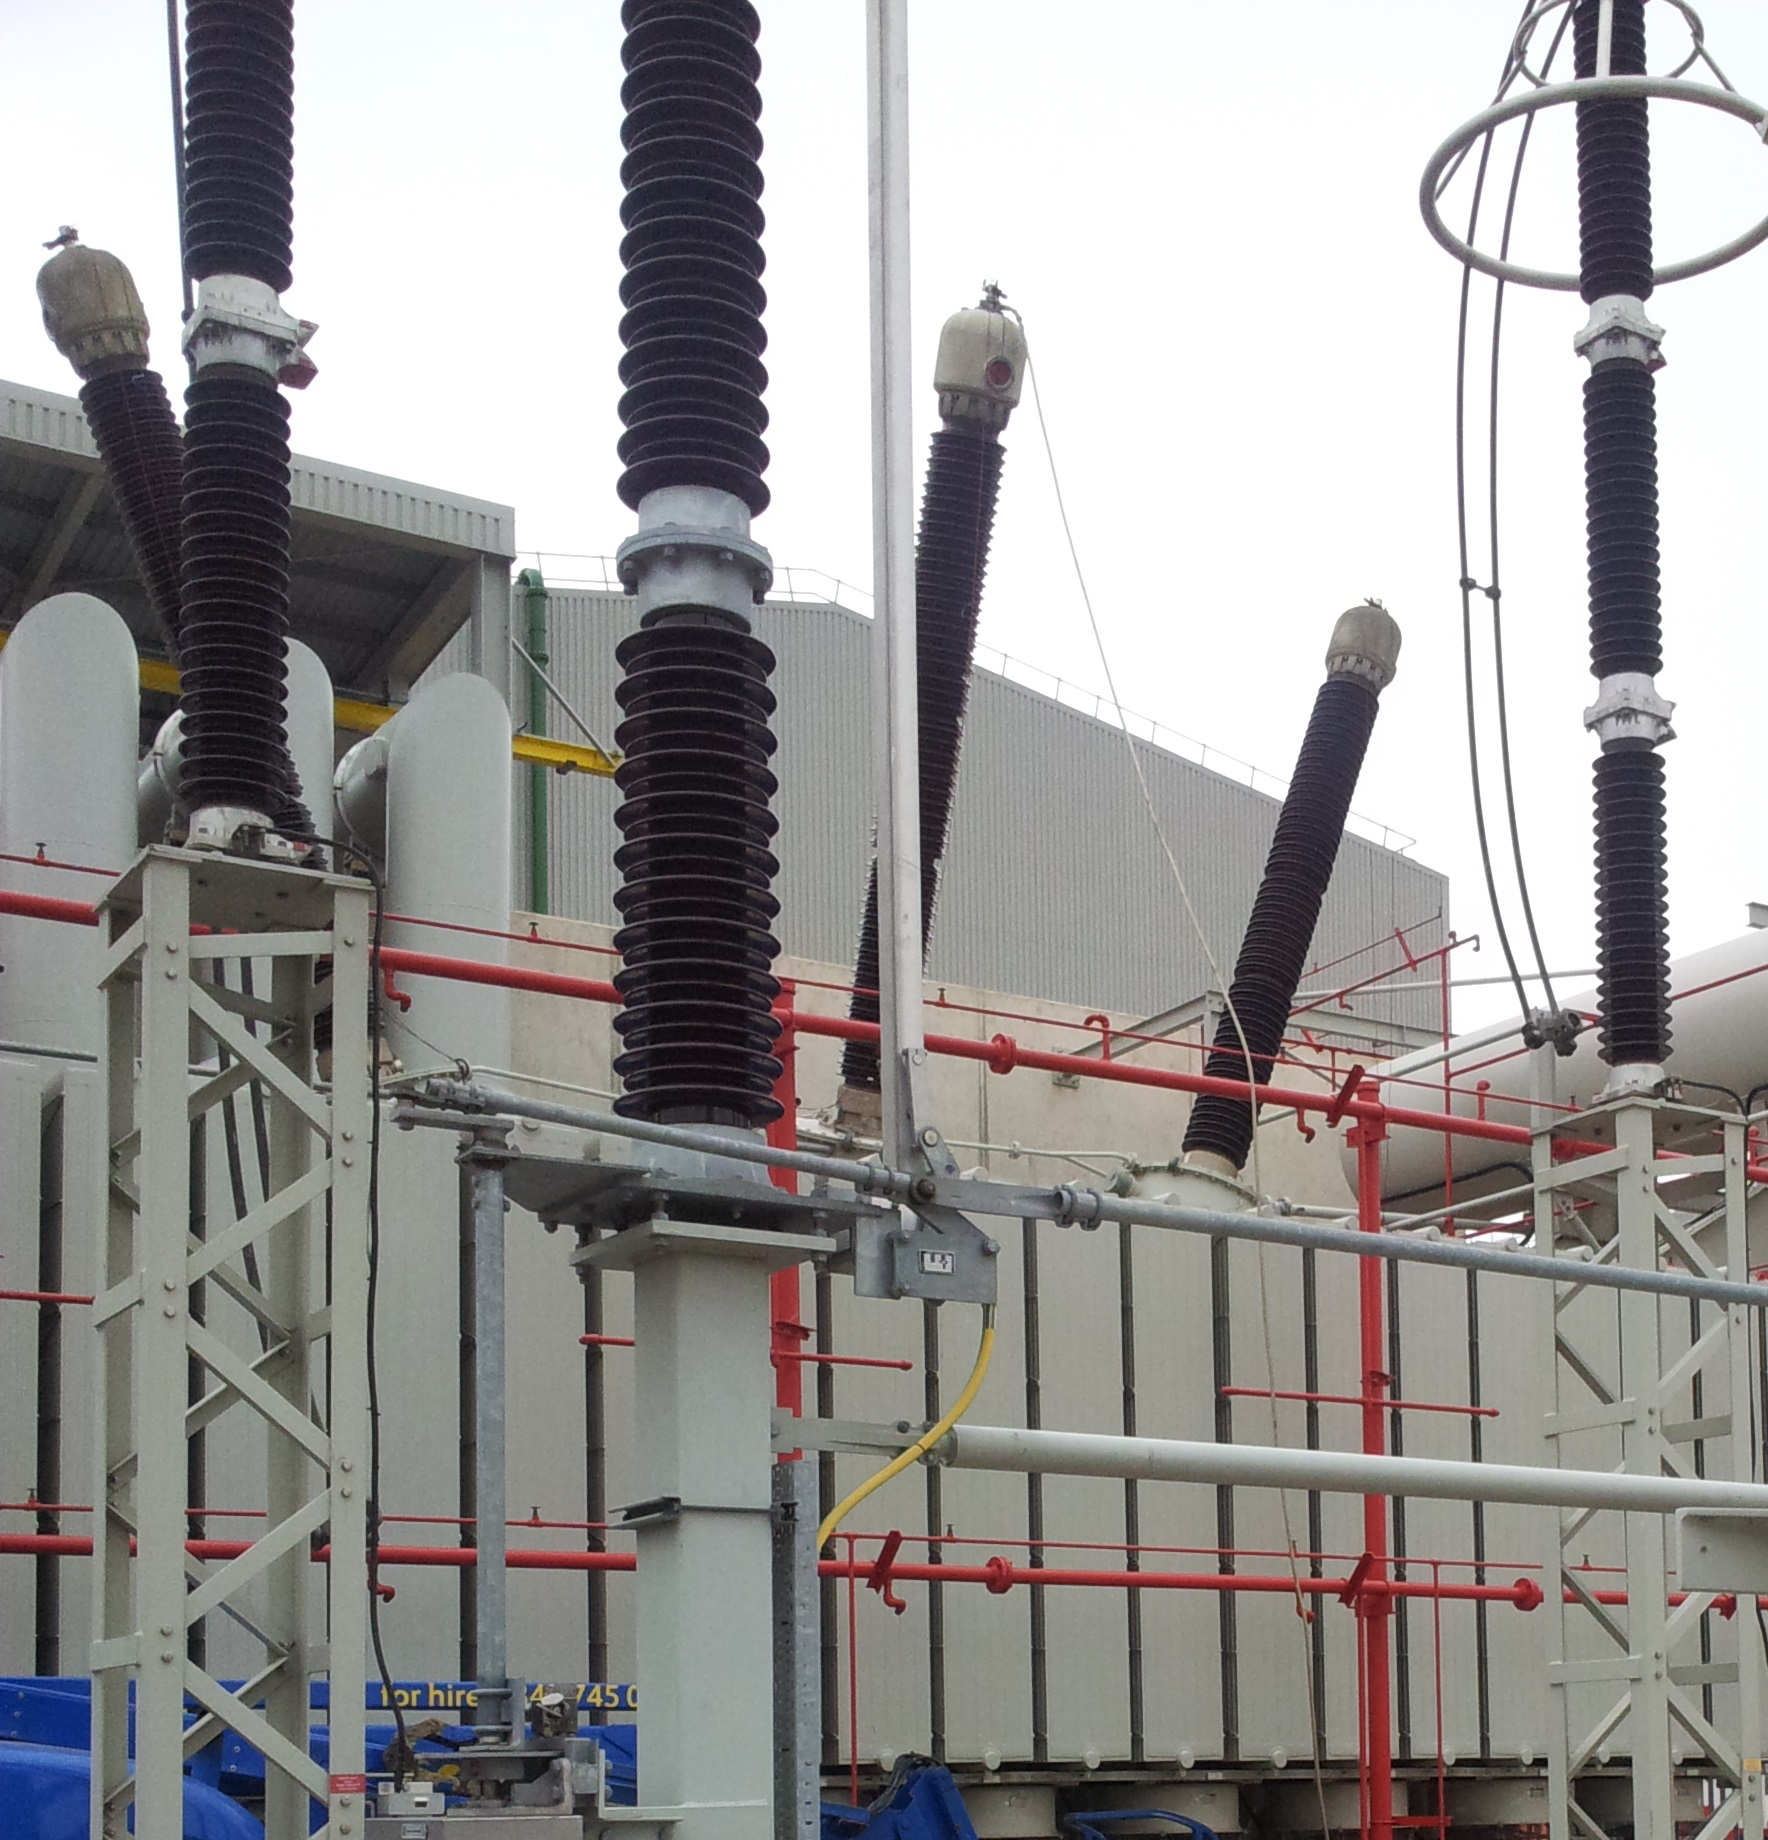
\includegraphics[height = 6cm]{StaythorpeHVBushingWide.jpg} 
	\label{Figure:Bush2}
  }
\caption{High Voltage Bushings on the 400kV Transformers at Staythorpe CCGT Power Station, Newark, UK (Taken by TJS)}
  \label{Figure:BothBushPics}
\end{figure}

